\section{Data}
\label{sec:data}
``The most satisfactory sampling design for structural analysis is a saturation sample of the entire universe or population; 
however, this alternative is clearly not feasible for large social structures'' 

\begin{flushright}
--- \textit{M.P. Allen, 1974}~\cite{Allen1974}
\end{flushright}

\subsection{Data description}
The data from this project was extracted from Orbis.
Orbis contains standardized information about 200 million firms and 100 million people. 
The firm data includes economic indicators (such as turnover, employee number, profit ratios or sector),
as well as 90 million ownership ties.
The directors data includes biographic information (such as name, education, nationality or gender), 
as well as 151 million position information,
indirectly creating 1,000 million interlocks.

The first step of the project consists on downloading, structuring and storing the data (months 1-4), quantifying the quality of the data (months 4-7) and assessing the effect on the results (months 8-9). For brevity we will skip most the details of the quality assessment. Figure ~\ref{fig:qual}A compares the number of companies in Orbis with the OECD. We can see that the quality is extremely good for large companies, but relatively bad for small companies. Importantly, the companies in Figure ~\ref{fig:qual}A are those with revenue and employment information (~60 million instead of 200). This is, most companies are in the database, but without financial information. 

We developed a two-step approach to assess the quality of the data. In the first step, we developed interactive visualizations to rapidly explore the data \footnote{\url{https://github.com/uvacorpnet}}. The results showed that richer countries (measured by GDP per capita) have larger companies and better coverage. The visualizations also showed that the observed average revenue for the companies in a country depends on the coverage. Those with higher coverage include also small companies, decreasing the `average' company. In the second step, we characterized the data and extrapolate the quality to other countries. The distributions of revenue for a country follow a lognormal distribution, thus can be defined using two parameters (loc and scale). Moreover, the scale is fixed for all countries and the loc can be estimated using macro-economic indicators. This allows to quantify the type of missing companies (Fig. ~\ref{fig:qual}B). In the next month I will assess the effect of this in network measures.

\begin{figure}
\begin{center}
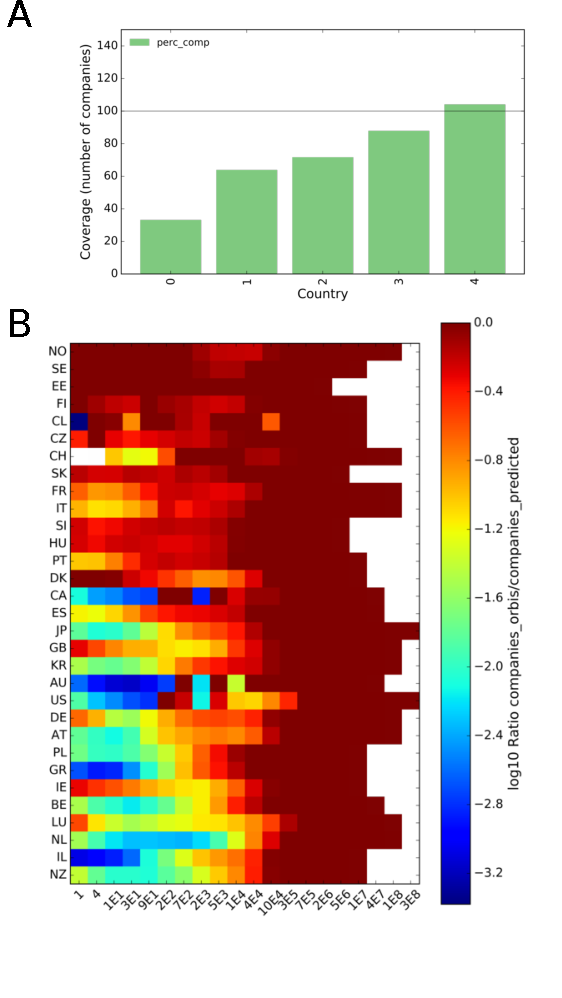
\includegraphics[width=.5\textwidth]{qual.pdf}
\caption{Global network of interlocking directorates. Color indicates communities -- i.e. cities that do business together within each other more often than with others.}
\label{fig:qual}
\end{center}
\end{figure}

\subsection{Data bias}

The concept of interlock comes not without problems. We want to measure relationships between companies. However it is not clear that formal interlocks --~those occurring by people sitting together on boards -- are more important than interlocks created by directors being part of the same social clubs or the same families. By restricting ourselves to formal interlocks we may be missing an important part of the corporate network. However, we expect to capture a significant part of the relations between companies.



In terms of internal validity, the concept of interlocks is captured in the data when one director holds positions in two companies. There are some problems with internal validity. Firstly, it’s not clear that we can separate administrative ties (mainly within corporate groups) from directorate ties (across corporate groups). This is so because the data providers from some countries (including the US) do not always state the type of position that a person holds.

External validity and reliability are intimately related in my case. Since I’m studying global data, I can generalize only if my data has high quality. If my data is good everybody can use the same methods and obtain the same results.[they can do that also if the data is bad, but of course you are right to want good data; you should look into the concepts of (internal) validity, reliability, and generalizability again – you have not fully understood them] 

Instead of talking about validity and reliability I will talk about completeness (how much of the data we have), bias (is our sample a random sample) and accuracy (is the data we have true). They are related to the concepts of validity and reliability and I believe they are more helpful in my discussion. I have extracted data about companies, with economic and geographic information about the company; and directors data, with information about people and the positions they hold.

Company data
1. Bias and completeness: We have assessed the bias and completeness of the data. We compared Orbis data with OECD data and found that small companies are underrepresented but large companies are always present. Moreover, we developed a method to use the economic data associated to each company to extrapolate the completeness to other countries. In general, Scandinavian countries have the highest quality (very complete and fairly unbiased), while poor countries have very bad data, although their biggest companies are present.
We can now use our method to reconstruct missing data and assess the effect of including it. We expect the effect to be small since small companies are not usually connected in the network -- for example the owner of a small shop is not likely to sit in the board of directors of any company.
[this means that there is bias, but you can assess the direction of the bias: it will lead you to find more interlockedness than there really is; this is important information; it is a problem if you want to make the case that there is a lot of interlockedness, because then you are facing a situation in which your data is biased in a way that  helps you prove yourself right; in that case it is better to propose that interlockedness is low, and then be able to show that it is still high, even if small (non-interlocked) companies are underrepresented in the data]

(this is actually the first paper of my PhD. I chose to come up with a new idea for the tasks since I believe I can learn more from the discussion in a more social science paper).

2.  Accuracy: We have checked the accuracy of a random sample and the information in the database is almost always correct. However, there are some problems in this area. Some information providers send their data faster than others, which makes the information of some countries be outdated (usually up to one year). Moreover, large company generally are required to fill consolidated accounts, including in their reports the profits, employees and other economics of their subsidiaries.  This doubles the information for big companies. [this is not clearly written]

We have found a way to use the ownership relationship between companies to unconsolidate accounts. [good] For the companies with over 250 employees, we now have around 100\% of the expected numbers according to OECD data, while before we were almost doubling the numbers.[this is not clearly written]

Directors data
1. Bias and completeness: Based on manual inspection of a small sample of the data we found that some directors from small companies are missing. However, we will try to impute this data based on other economic factors (work in progress).[how is that possible?]

2.  Accuracy: The accuracy of the data is not great either. Large companies have extra directors that have already left the company. The position of directors in some countries is unspecified, meaning that we don’t know if they are administrative ties or not. We can remove administrative ties by using the ownership database. If a director has positions in a shareholder and a wholly owned subsidiary then we can filter that tie. The problem with this approach is that two subsidiaries that are wholly owned by company A may not have any ownership relationship between them, but they are still the same corporation. We need to think more about this problem and try different solutions.[related to my comment above, this means you are adapting your data pool to be able to stick to your original definition of interlocks]

In general, the way to assess validity and reliability in my paper is to assure good data quality. [data quality is only one source of validity; there are many more issues to consider to maximize the validity of your conclusions] We will do this by imputing the missing data and using this to produce confidence intervals of our metrics. Assessing data quality correctly, and analyzing the entire global network (instead of the top X firms) may allow us to give definite answers to many questions.
[your approach to your research is very much data-driven; while you are right to be excited about your data, as it is a rich source of information and can help you make many interesting claims, it is important to get your head out of the data, so to speak, and think strategically about the questions you want answered and the way to answer them]


In terms of operationalization, it is not clear that we can distinguish interlocking directorates from administrative ties. While the first are created by people with ability to decide or control decisions, in the second case the two `companies’ are not independent, but are part of the same structure.  Our data does not specify for some countries if the person creating the relationship is a director -- and therefore the relationship is a interlock -- or if the person is an administrative. However we expect to be able to correct this by using ownership information about companies. Relationships between companies that are accompanied by an ownership relationship can be discarded. 
